\documentclass{beamer}
\usepackage{amssymb,amsmath,amsthm,amsaddr}
\usepackage{thmtools}
\usepackage{thm-restate}

\usepackage{tikz,pgfplots,pgfplotstable}
\pgfplotsset{compat=1.9} % set to 1.8 to get old behaviour

%% %% % Graphics:
%% \usepackage[final]{graphicx}
\usepackage{graphicx} % use this line instead of the above to suppress graphics in draft copies
\usepackage{wrapfig}
%\usepackage{graphpap} % \defines the \graphpaper command
\usepackage[T1]{fontenc} % Use 8-bit encoding that has 256 glyphs
\usepackage[english]{babel} % English language/hyphenation


\usepackage{cite}
% makes color citations
\usepackage[colorlinks=true,urlcolor=blue,citecolor=red,linkcolor=red,bookmarks=true]{hyperref}
\usepackage{url}
\usepackage{color}
\usepackage{paralist}
%% \usepackage{graphics} %% add this and next lines if pictures should be in esp format
%% \usepackage{epsfig} %For pictures: screened artwork should be set up with an 85 or 100 line screen
\usepackage{epstopdf} 

%% From slides file
\usepackage{booktabs} % Allows the use of \toprule, \midrule and \bottomrule in tables
\usepackage[normalem]{ulem}
\usepackage{xcolor}
%\usepackage{algorithm}
%\usepackage[noend]{algpseudocode}
\usepackage{proof-at-the-end}

% Indent first line of each section:
\usepackage{indentfirst}

%% %% % Fonts and symbols:
\usepackage{amsfonts}


%% % Formatting tools:
%% %\usepackage{relsize} % relative font size selection, provides commands \textsmalle, \textlarger
%% %\usepackage{xspace} % gentle spacing in macros, such as \newcommand{\acims}{\textsc{acim}s\xspace}

%% % Page formatting utility:
%% \usepackage{geometry}
%% %\usepackage[margin=0.1in]{geometry}


%% Place here your \newcommand's and \renewcommand's. Some examples already included.
%\renewcommand{\le}{\leqslant}
%\renewcommand{\ge}{\geqslant}
%\renewcommand{\emptyset}{\ensuremath{\varnothing}}
%\newcommand{\ds}{\displaystyle}
\newcommand{\R}{\ensuremath{\mathbb{R}}}
%\newcommand{\Q}{\ensuremath{\mathbb{Q}}}
%\newcommand{\Z}{\ensuremath{\mathbb{Z}}}
%\newcommand{\N}{\ensuremath{\mathbb{N}}}
%\newcommand{\T}{\ensuremath{\mathbb{T}}}
%\newcommand{\B}{\mathcal{B}}
\newcommand{\eps}{\varepsilon}
%\newcommand{\closure}[1]{\ensuremath{\overline{#1}}}
\newcommand{\M}{\mathcal{M}}

\newcommand{\ep}{\varepsilon}
%\newcommand{\eps}[1]{{#1}_{\varepsilon}}
\newcommand{\bs}{\boldsymbol}
\newcommand{\der}{\text{\textup{d}}}
\newcommand{\coder}[1]{\texttt{#1}}
\newcommand{\inner}[2]{#1 \cdot #2}
\newcommand{\var}{\textup{Var}}
\newcommand{\corr}{\textup{Corr}}
\newcommand{\cov}{\textup{Cov}}
\newcommand{\diag}{\textup{diag}}
%% \newcommand{\dom}{\mathcal{D}om}
%% \newcommand{\note}[1]{{\textcolor{blue}{#1}}}
%% \newcommand{\A}[1]{{\textcolor{cyan}{\noindent Answer: #1}}}
%\newcommand{\reftwo}[1]{{\textcolor{green}{#1}}}
%\newcommand{\refthree}[1]{{\textcolor{red}{#1}}}
%% \newcommand{\refthree}[1]{{\color{red} #1}}
%% \newcommand{\reftwo}[1]{{\color{green} #1}}



%% \newcommand{\precop}{\mathcal{L}}
%% \newcommand{\precmat}{\mathbf{L}}
%% \newcommand{\Op}{\mathcal{A}}
%% \newcommand{\OpDir}{\mathcal{A}_{\textup{Dirichlet}}}
%% \newcommand{\OpNeu}{\mathcal{A}_{\textup{Neumann}}}
%% \newcommand{\covop}{\mathcal{C}}
%% \newcommand{\lag}{\mathcal{L}}
%% \newcommand{\n}{\boldsymbol{n} }
%% \newcommand{\dn}{\partial \n }
\newcommand{\x}{\mathbf{x}}
\newcommand{\y}{\mathbf{y}}
%% \newcommand{\z}{{\boldsymbol{z}}}
%% \newcommand{\kxmy}{ \kappa \| \x - \y \| }
%% \newcommand{\xmy}{ \| \x - \y \| }
%% \newcommand{\proj}{\mathcal{P}}
%% \newcommand{\kr}{\kappa r}
%% \newcommand{\ivar}{\text{IntVar}}

%% \newcommand{\K}{\mathbb{K}}
\newcommand{\hil}{\mathcal{H}}
%% \newcommand{\ban}{\mathcal{B}}
\newcommand{\hilp}{\mathcal{H}_p}
\newcommand{\hilo}{\mathcal{H}_o}
\newcommand{\obs}{\mathcal{O}}
\newcommand{\pobs}{\mathcal{P}}
\newcommand{\fwd}{\mathcal{F}}
%% \newcommand{\tru}{\fwd_{\textup{True}}}
%% \newcommand{\err}{\fwd_{\textup{Error}}}

\newcommand{\obsm}{\widehat{\obs}}
\newcommand{\Sigmam}{\widehat{\Sigma}}
\newcommand{\postcovm}{\widehat{\Gamma_{\textup{post}}}}
\newcommand{\uu}{\mathbf{u}}
\newcommand{\tar}{\Psi}
\DeclareMathOperator*{\argmin}{arg\,min}
\DeclareMathOperator*{\argmax}{arg\,max}

% Definitions for second chapter
\newcommand{\data}{\mathbf{d}}
\newcommand{\param}{\mathbf{m}}
\newcommand{\sspar}{\param_{\textup{SmallScale}}}
\newcommand{\normal}{\mathcal{N}}
\newcommand{\pr}{\mu_{\textup{pr}}} %Prior measure
\newcommand{\post}{\mu_{\textup{post}}^{\data, \obs}} % Posterior measure
\newcommand{\prmean}{\param_{\textup{pr}}} % Prior mean
\newcommand{\postmean}{\param_{\textup{post}}} % Posterior mean
\newcommand{\postcov}{\Gamma_{\textup{post}}} % Posterior covariance
\newcommand{\prcov}{\Gamma_{\textup{pr}}} % Prior covariance
\newcommand{\modcov}{\Gamma_{\textup{model}}} % Model covariance
\newcommand{\tmp}{\mathcal{G}}
\newcommand{\meas}{\mathbf{o}}
\newcommand{\ev}{\mathbf{e}} % eigenvector 
\newcommand{\func}{\mathbf{a}}
\newcommand{\tr}[1]{\textup{tr}\left \{#1 \right \} }
\newcommand{\ttr}[1]{\textup{tr}\ #1}
\newcommand{\rank}{\textup{rank}\ }
\newcommand{\des}{\eta} % vector of design parameters
\newcommand{\sigsqr}{\sigma^2}
%\newcommand{\acim}{\textsc{acim}\xspace}
%\newcommand{\acims}{\textsc{acim}s\xspace}


%% %% \newcommand\numberthis{\addtocounter{equation}{1}\tag{\theequation}}
%% %% %%
%% %% %% Place here your \newtheorem's:
%% %% %%
\newtheorem{theorem}{Theorem}
\newtheorem{definition}{Definition}

%% %% %% Some examples commented out below. Create your own or use these...
%% %% %%%%%%%%%\swapnumbers % this makes the numbers appear before the statement name.
%% %% %\theoremstyle{plain}
%% %% %\newtheorem{thm}{Theorem}[chapter]
\newtheorem{proposition}{Proposition}
\newtheorem{lemma}{Lemma}
\newtheorem{corollary}{Corollary}
%% %% % \newtheorem{observation}[theorem]{Observation}

%% %% %\theoremstyle{definition}
%% %% %\newtheorem{define}{Definition}[chapter]

%% %% %\theoremstyle{remark}
%% %% %\newtheorem*{rmk*}{Remark}
%% %% %\newtheorem*{rmks*}{Remarks}

%% %% %% Hack
%% %% \newcommand{\stkout}[1]{\ifmmode\text{\sout{\ensuremath{#1}}}\else\sout{#1}\fi}
%% %% \usepackage{cancel}

\usepackage{comment}% http://ctan.org/pkg/comment
%% %% %\excludecomment{proof}
%% \excludecomment{figure}
%% \let\endfigure\relax


\overfullrule=0pt


\begin{document}


% Slide 1: Title
\begin{frame}
\frametitle{Measurement Clusterization in Bayesian D-optimal Designs in Infinite Dimensions}
\end{frame}

% Slide 2: Forward problem
\begin{frame}
\frametitle{Forward problem}
% Example 1: Ball toss
% Example 2: Flow field (placeholder for image)
% Example 3: Ink in water
\[
\fwd: \hilp \to \hilo
\]
\end{frame}

% Slide 3: Inverse problem
\begin{frame}
\frametitle{Inverse problem}
% Explain the inverse problems for the ball toss, flow field examples
% Argue that there are many valid solutions
% Explain that such problems are ill-posed
\end{frame}

% Slide 4: Toy example
\begin{frame}
\frametitle{Toy example: 1D heat equation}
% Present the 1D heat equation with homogeneous Dirichlet boundary condition

\begin{subequations}\label{eq:heat equation}
  \begin{alignat}{2}
    u_t &= \Delta u &&\qquad \text{in } [0,1] \times [0,\infty),\\
      u &= 0 &&\qquad \text{on } \{0, 1\} \times [0,\infty),\\
        u &= u_0 &&\qquad \text{on }[0,1] \times \{0\}.
  \end{alignat}
\end{subequations}

\end{frame}

% Slide 5: Solving inverse problems
\begin{frame}
\frametitle{Measurements}
% Show "sensor" and discuss measurement placement
\begin{equation*}%\label{eq:O}
  \obs u = (\meas_1(u), \dots, \meas_m(u) )^t \in \R^m,\ u \in \hilo.
\end{equation*}

% Introduce D-Optimality heuristically
\end{frame}

% Slide 6: Prior and posterior measures
\begin{frame}
\frametitle{Prior and posterior}
% Introduce prior measure $\mu_{\text{pr}}$ and posterior measure $\mu_{\text{post}}$
% Define KL-divergence and provide an intuitive explanation
\end{frame}

% Slide 7: Gaussian measures on Hilbert spaces
\begin{frame}
\frametitle{Gaussian measures on Hilbert spaces}
% Define Gaussian measure
% Show a 2D example with iso-density lines and projections
% Introduce notation for mean $\mathbf{m}$ and covariance $\Gamma$
\end{frame}

% Slide 8: Recap and notation summary
\begin{frame}
\frametitle{Recap and notation summary}
% Summarize notation:
\begin{itemize}
\item Forward operator \(\fwd: \hilp \to \hilo\)
\item Parameter space $\hilp$.
\item Observation space $\hilo$.
\item Observation operator $\obs: \hilo \to \mathbb{R}^m$
\item Prior measure $\pr \sim \mathcal{N}(0, \prcov)$.
\item Posterior measure $\post \sim \mathcal{N}(0, \postcov)$.
\end{itemize}
%% 1D heat equation
\end{frame}

% Slide 9: Formalism of inverse problems
\begin{frame}
  \frametitle{Formalism of inverse problems}
  \begin{align}\label{eq:inverse problem}
    \data := \obs \fwd \param + \eps
  \end{align}
  
  % Present the entire formalism of inverse problems from the paper, for zero model error
\end{frame}

% Slide 10: D-optimality criterion
\begin{frame}
  \frametitle{D-optimality criterion}
  \begin{theorem}[Alexanderian, Gloor, Ghattas \cite{AlexanderianGloorGhattas14}]\label{thm:d optimality}
    Let \(\pr = \normal(\prmean,\prcov)\) be a Gaussian prior on \(\hilp\)
    and let \(\post = \normal(\postmean,\postcov)\) the posterior measure
    on \(\hilp\) for the Bayesian linear inverse problem \(\data = \obs
    \fwd\param +  \eps\). Then
    \begin{align}\label{eq:objective}
      \begin{split}
        \tar( \obs) :&= \mathbb{E}_{\data}\left [ D_{\text{KL}} (\post || \pr ) \right ] \\
        % 
        % 
        % 
        &= \frac12 \log \det 
        ( I + \sigma^{-2} \prcov^{1/2}  \fwd ^* \obs^* \obs \fwd \prcov^{1/2}).
      \end{split}
    \end{align}
  \end{theorem}

% Show the D-optimality criterion from Alexanderian et al.
% Assume linear forward operator and linear observation operator
% Provide intuition about the log det of quotient of posterior and prior covariance/precision operators
\end{frame}

\begin{frame}
  \begin{definition}\label{def:d optimality}
  We say \(\obs^{\star}\) is \emph{D-optimal} if \(\obs^{\star} =
  \argmax_{\obs} \tar(\obs)\), where entries of \(\obs \in (\hilo^*)^m\)
  are constrained to some allowed set of measurements in \(\hilo^*\).
\end{definition}

  \end{frame}
% Slide 11: Sensor clusterization
\begin{frame}
\frametitle{Problem: Sensor clusterization}
\begin{figure}
    \centering
    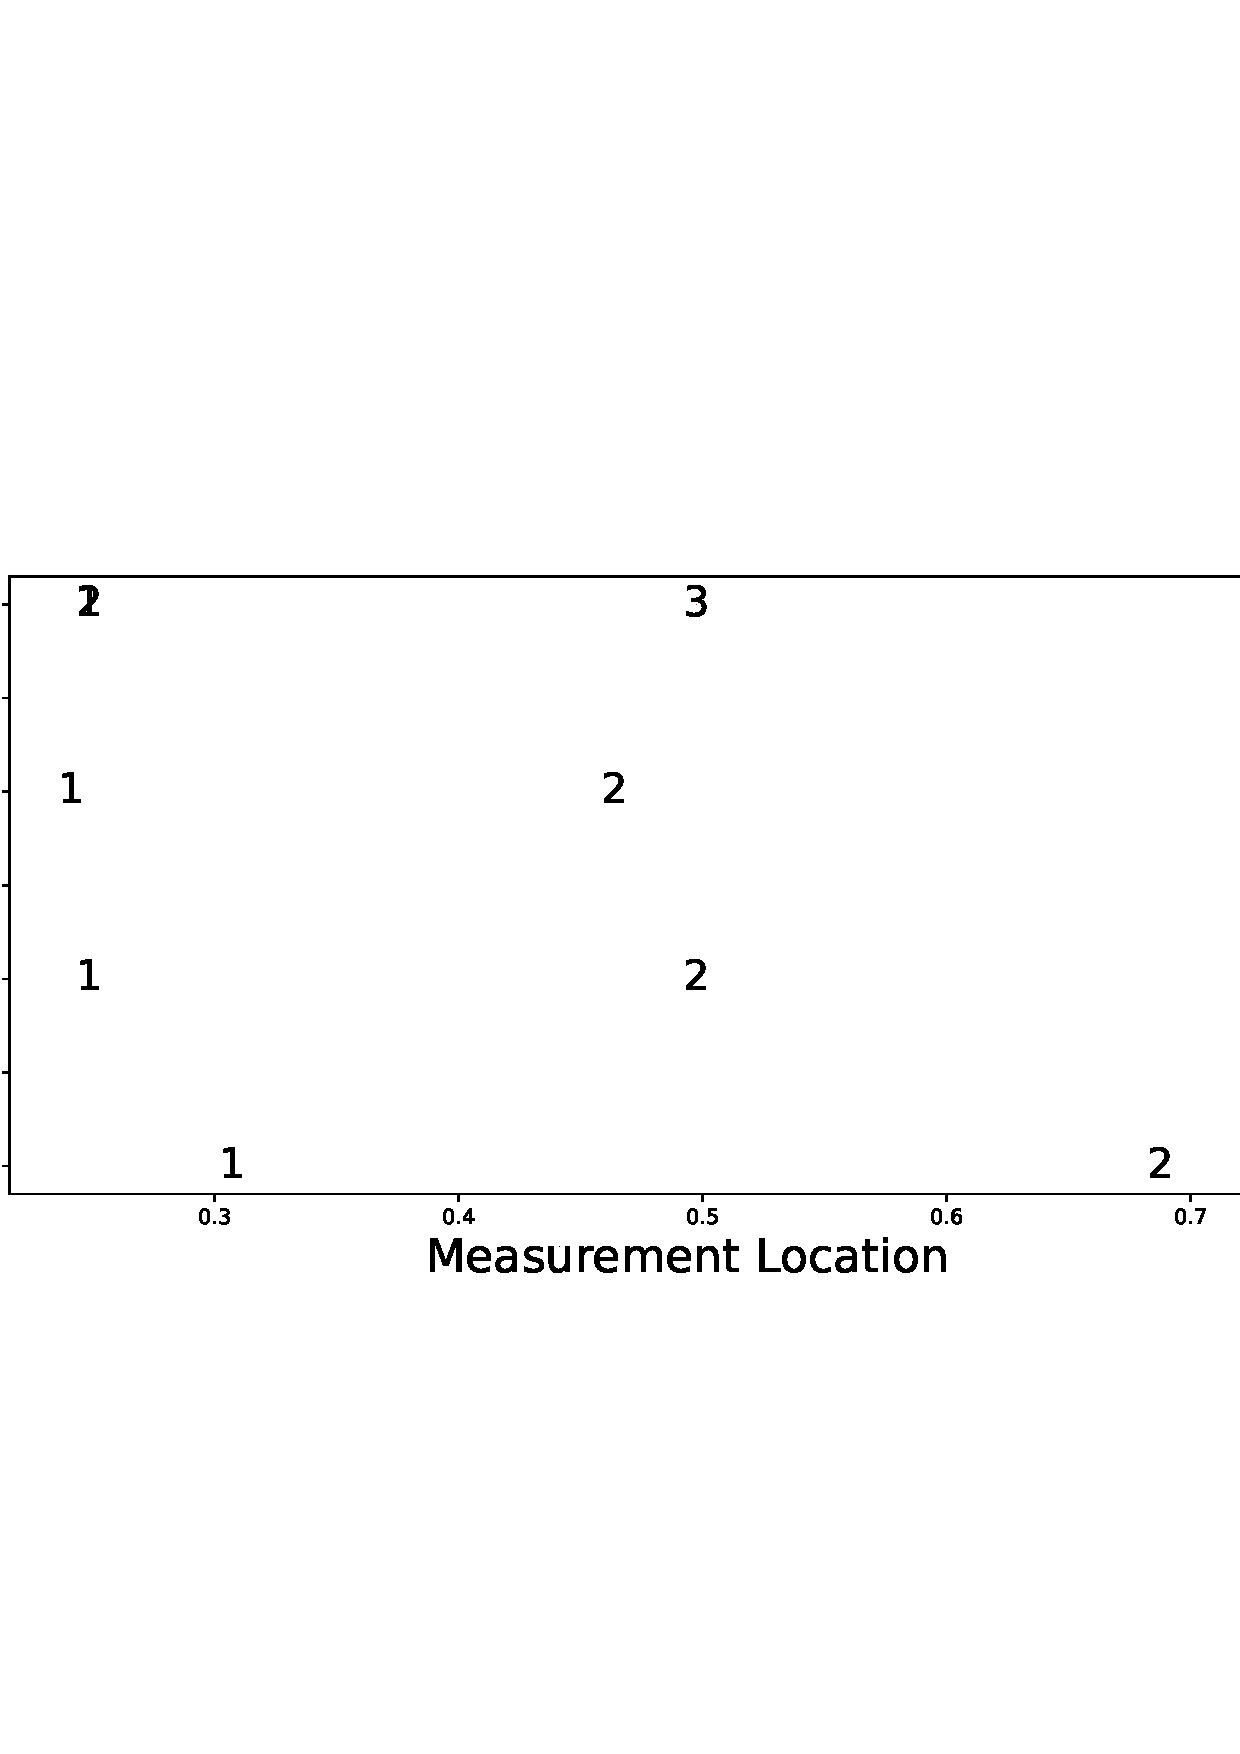
\includegraphics[height=0.5\textwidth]{example.pdf}
  %%   \caption{Measurement clusterization for optimal designs when
  %%     inverting for the initial condition of the 1D heat equation (see
  %%     supplementary material for details). Measurement locations were
  %%     chosen according to the Bayesian D-optimality criterion of
  %%     Theorem \ref{thm:d optimality}. Measurement locations are
  %%     plotted over the computational domain \(\Omega = [0, 1]\)
  %%     (x-axis), for varying numbers of measurements (y-axis). The
  %%     colored numbers are measurement indices, plotted for visual
  %%     clarity. Measurement clusterization already occurs for three
  %%     measurements: the second measurement (red) is overlaid with the
  %%     third (green). For five measurements, first (blue) and second
  %%     (red) measurements are clustered, as well as the fourth (black)
  %%     and the fifth (magenta).}
  %% \label{fig:clusterization illustration}
\end{figure}

% Discuss sensor clusterization in the 1D heat equation example
% Show figure from the paper (placeholder for figure)
\end{frame}

% Slide 12: Avoiding clusterization
\begin{frame}
\frametitle{Avoiding clusterization}
\begin{itemize}
\item Model correlation
\item Choose from a finite set of sensor locations
\end{itemize}
\end{frame}

% Slide 13: Main questions
\begin{frame}
\frametitle{Main questions}
% Present the main questions from the introduction of the paper
\begin{itemize}
\item Why does imposing correlations between observations alleviate
measurement clusterization?
%
\item Is measurement clusterization a generic phenomenon?
%
\item And, most importantly: Why does measurement clusterization occur?
% How do we tackle this problem?
\end{itemize}
\end{frame}

% Slide 14: Proposed approach
\begin{frame}
\frametitle{A "generic" inverse problem}
Recall definitions

\begin{align}\label{eq:inverse problem}
    \data := \obs \fwd \param + \eps
\end{align}

%% \begin{align}\label{eq:objective}
%%   \begin{split}
%%     \tar( \obs) &= \frac12 \log \det 
%%     ( I + \prcov^{1/2}  \fwd ^* \obs^* \Sigma^{-1} \obs \fwd \prcov^{1/2}).
%%   \end{split}
%% \end{align}

% Discuss the main obstacle: the measurement operator
% Impose unit-norm constraints
% Explain that sensors have a unit inf-norm (show example)
% Show relevant equation from the paper
\end{frame}

% Slide 15: Constrained optimization problem
\begin{frame}
\frametitle{Constrained optimization problem}
% Restate the optimization criterion from Alexandrian et al.'s theorem
% Restate the unit norm constraints
% Pose the problem as a constrained optimization problem
% Ask the audience how to solve constrained optimization problems (Lagrange multipliers)
Let The D-optimality design criterion
\cite{AlexanderianGloorGhattas14}:
\begin{align*}
  \begin{split}
    \tar(\obs) %:&= \mathbb{E}_{\data}\left [ D_{\text{KL}} (\post || \pr ) \right ] \\
    % 
    % 
    % 
    &= \frac12 \log \det ( I + \sigma^{-2} \prcov^{1/2} \fwd ^*
    \obs^* \obs \fwd \prcov^{1/2}), 
  \end{split}
\end{align*}
The constrained optimization problem of D-Optimal designs entails finding
\begin{equation*}
  \obs = \argmax_{\|\meas_j\| = 1, j=1,\dots,m}\tar(\obs),
\end{equation*}
\end{frame}

% Slide 16: Necessary conditions for optimality
\begin{frame}
\frametitle{Necessary conditions for optimality}
% Present the nonlinear eigenvalue problem for the vanishing model error case
% Explain why it is called a "nonlinear" eigenvalue problem

\begin{theorem}[Necessary conditions for D-Optimality]\label{thm:constrained}
  Let:
  \begin{equation*}
    \obs^{\star} &= \tar(\obs).
    \text{subject to: } \|\meas_j\| &= 1\ \text{ for } j=1,\dots,m
  \end{equation*}
  
  Then:
  \begin{equation*}
    \fwd \postcov \fwd^* \obs^*  \Sigma^{-1}  = \obs^* \Xi, 
  \end{equation*}
  where $\Xi \in \mathbb{R}^{m \times m}$ is diagonal.
\end{theorem}

\end{frame}

% Slide 17: Lemma 17
\begin{frame}
\frametitle{Lemma 17}
% State Lemma 17 (placeholder for the actual lemma)
\end{frame}

% Slide 18: Main theorem
\begin{frame}
\frametitle{Main theorem}
% State the main theorem
\end{frame}

% Slide 19: Main theorem explanation
\begin{frame}
\frametitle{Main theorem explanation}
% Explain the main theorem using a graph and three graduated lab cylinders
\end{frame}

% Add the remaining slides here
% ...

\end{document}
